\documentclass[12pt,]{article}
\usepackage[left=1in,top=1in,right=1in,bottom=1in]{geometry}
\newcommand*{\authorfont}{\fontfamily{phv}\selectfont}
\usepackage[]{mathpazo}


  \usepackage[T1]{fontenc}
  \usepackage[utf8]{inputenc}



\usepackage{abstract}
\renewcommand{\abstractname}{}    % clear the title
\renewcommand{\absnamepos}{empty} % originally center

\renewenvironment{abstract}
 {{%
    \setlength{\leftmargin}{0mm}
    \setlength{\rightmargin}{\leftmargin}%
  }%
  \relax}
 {\endlist}

\makeatletter
\def\@maketitle{%
  \newpage
%  \null
%  \vskip 2em%
%  \begin{center}%
  \let \footnote \thanks
    {\fontsize{18}{20}\selectfont\raggedright  \setlength{\parindent}{0pt} \@title \par}%
}
%\fi
\makeatother




\setcounter{secnumdepth}{0}


\usepackage{graphicx,grffile}
\makeatletter
\def\maxwidth{\ifdim\Gin@nat@width>\linewidth\linewidth\else\Gin@nat@width\fi}
\def\maxheight{\ifdim\Gin@nat@height>\textheight\textheight\else\Gin@nat@height\fi}
\makeatother
% Scale images if necessary, so that they will not overflow the page
% margins by default, and it is still possible to overwrite the defaults
% using explicit options in \includegraphics[width, height, ...]{}
\setkeys{Gin}{width=\maxwidth,height=\maxheight,keepaspectratio}

\title{ChangeMyView: Can Moral Appeals Facilitate Compromise?\thanks{\textbf{Version}: February 27, 2018 --- PLEASE DO NOT CITE OR
REDISTRIBUTE WITHOUT PERMISSION.}  }



\author{\Large Patrick W. Kraft\vspace{0.05in} \newline\normalsize\emph{Stony Brook University}  }


\date{}

% sans serif font
%\renewcommand{\familydefault}{\sfdefault}

% Computer Modern Bright font (sans serif)
%\usepackage{cmbright}
%\usepackage[T1]{fontenc}


\usepackage{titlesec}

\titleformat*{\section}{\normalsize\bfseries}
\titleformat*{\subsection}{\normalsize\itshape}
\titleformat*{\subsubsection}{\normalsize\itshape}
\titleformat*{\paragraph}{\normalsize\itshape}
\titleformat*{\subparagraph}{\normalsize\itshape}


\usepackage{natbib}
\bibliographystyle{/home/patrick/Dropbox/Uni/Lit/apsr2006}
\usepackage[strings]{underscore} % protect underscores in most circumstances



\newtheorem{hypothesis}{Hypothesis}
\usepackage{setspace}

\makeatletter
\@ifpackageloaded{hyperref}{}{%
\ifxetex
  \PassOptionsToPackage{hyphens}{url}\usepackage[setpagesize=false, % page size defined by xetex
              unicode=false, % unicode breaks when used with xetex
              xetex]{hyperref}
\else
  \PassOptionsToPackage{hyphens}{url}\usepackage[unicode=true]{hyperref}
\fi
}

\@ifpackageloaded{color}{
    \PassOptionsToPackage{usenames,dvipsnames}{color}
}{%
    \usepackage[usenames,dvipsnames]{color}
}
\makeatother
\hypersetup{breaklinks=true,
            bookmarks=true,
            pdfauthor={Patrick W. Kraft (Stony Brook University)},
             pdfkeywords = {Moral Foundations, Attitude Change, Persuasion, Compromise},  
            pdftitle={ChangeMyView: Can Moral Appeals Facilitate Compromise?},
            colorlinks=true,
            citecolor=blue,
            urlcolor=blue,
            linkcolor=magenta,
            pdfborder={0 0 0}}
\urlstyle{same}  % don't use monospace font for urls

% set default figure placement to htbp
\makeatletter
\def\fps@figure{htbp}
\makeatother



% add tightlist ----------
\providecommand{\tightlist}{%
\setlength{\itemsep}{0pt}\setlength{\parskip}{0pt}}

\begin{document}
	
% \pagenumbering{arabic}% resets `page` counter to 1 
%
% \maketitle

{% \usefont{T1}{pnc}{m}{n}
\setlength{\parindent}{0pt}
\thispagestyle{plain}
{\fontsize{18}{20}\selectfont\raggedright 
\maketitle  % title \par  

}

{
   \vskip 13.5pt\relax \normalsize\fontsize{11}{12} 
\textbf{\authorfont Patrick W. Kraft} \hskip 15pt \emph{\small Stony Brook University}   

}

}








\begin{abstract}

    \hbox{\vrule height .2pt width 39.14pc}

    \vskip 8.5pt % \small 

\noindent The American electorate is becoming increasingly polarized. According to
research in moral psychology, these growing disagreements between
liberals and conservatives can be attributed to fundamental differences
in the moral frameworks that shape individual ideology. Indeed, scholars
suggest that ideologues would be more likely to reach compromise if both
sides spoke the same ``moral language.'' While this implicit assumption
has intuitive appeal, it remains largely untested empirically. Drawing
on a unique dataset from the online discussion board \emph{Reddit}, this
paper examines how moral appeals can affect individual persuasion and
the likelihood of agreement and consensus building through deliberation.


\vskip 8.5pt \noindent \emph{Keywords}: Moral Foundations, Attitude Change, Persuasion, Compromise \par

    \hbox{\vrule height .2pt width 39.14pc}



\end{abstract}


\vskip 6.5pt


\noindent \doublespacing Recent years have witnessed a resurgence in partisan polarization in the
United States. Politically engaged citizens hold more diverging policy
views, are more ideologically extreme, and exhibit stronger negative
affect towards out-partisans than in the past
\citep{hetherington2001resurgent, abramowitz2008polarization, iyengar2012affect, mason2014disrespectfully, huddy2015expressive, iyengar2015fear}.
A growing literature in moral psychology---building on Moral Foundations
Theory---attributes this divide (at least partially) to fundamental
differences in moral frameworks that guide liberal and conservative
thinking \citep[c.f.,][]{haidt2012righteous}. According to this
perspective, liberals focus on \emph{individualizing} moral foundations,
which include care/harm and fairness/cheating. Conservatives, on the
other hand, also emphasize the remaining \emph{binding} foundations of
loyalty/betrayal, authority/subversion, and sanctity/degradation
\citep{haidt2007morality, graham2009liberals}. Differential emphasis on
these moral dimensions is systematically related to attitudes towards a
wide variety of divisive political issues
\citep[e.g.][]{koleva2012tracing, kertzer2014moral, low2015moral},
personality traits like individual social dominance orientation (SDO)
and right-wing authoritarianism (RWA) \citep{federico2013mapping}, as
well as voting behavior \citep{franks2015using}. Overall, this body of
research suggests that liberals and conservatives endorse different
moral foundations and that these differences are related to political
attitudes, evaluations, and behavior.

An important implicit assumption that has been made repeatedly in this
literature is that liberals and conservatives would be more likely to
come to agreements \emph{if only they focused on the same moral
foundations}. For example \citet[365]{haidt2012righteous} concludes in
his book \emph{The Righteous Mind: Why Good People Are Divided by
Politics and Religion}: ``Once people join a political team, they get
ensnared in its moral matrix. They see confirmation of their grand
narrative everywhere, and it's difficult---perhaps impossible---to
convince them that they are wrong \emph{if you argue with them from
outside of their matrix}'' (emphasis added). In an different article,
\citet[1040]{graham2009liberals} contend that their findings ``help
explain \emph{why liberals and conservatives disagree on so many moral
issues} and often find it hard to understand how an ethical person could
hold the beliefs of the other side: Liberals and conservatives
\emph{base their moral values, judgments, and arguments on different
configurations} of the five foundations.'' The underlying assumption
that emphasizing the same foundations can facilitate compromise has
important implications---especially in our current political
environment. Somewhat surprisingly, however, it has never been subjected
to a direct empirical test.

There are reasons to believe that compromise is still difficult---and
potentially even further impeded---if individuals argue on the basis of
the same set of moral foundations. \citet{skitka2005moral}, for example,
provide a different theoretical perspective than MFT by conceptualizing
moralization as a unique feature of attitude strength. According to this
view, moral convictions are perceived as ``absolutes, or universal
standards of truth that others should also share''
\citep[269]{skitka2010psychology}. As such, they combine the following
attributes: they are viewed by individuals as applying to everyone
(universality), they do not require an immediate underlying rationale
but are rather seen as facts about the world (objectivity), they can be
independent of authority and group norms (autonomy), they elicit strong
emotional reactions, and they have an inherent motivational quality
(motivation/justification) \citep{skitka2010psychology}. Building on
this work, \citet{ryan2014reconsidering} argued that moral convictions
are not restricted to issues that are traditionally perceived as
``moral,'' such as abortion or same-sex marriage, but can also include
other issues such as economic policies. The degree of moral conviction
may therefore vary between individuals as well as across issues.
\citet{ryan2014reconsidering} further showed that the propensity to
moralize---i.e.~the tendency to view an issue as a question of ``right
and wrong''---is related to political participation, extreme political
attitudes, arousal of negative emotions, and hostility. In a subsequent
study, \citet{ryan2016no} suggested that moralization as a distinct
characteristic of attitude intensity reorients behavior from maximizing
gains to the general adherence to rules. Across multiple studies, the
author showed that this tendency translates into stronger opposition to
compromise about political issues and decreased support for compromising
politicians. These patterns should also translate into attitudes
towards---and interactions with---others who hold opposing views.
Indeed, moral conviction has been shown to be related to stronger
preferences for social distance from (and hostility towards)
attitudinally dissimilar others and lower cooperativeness in groups
holding heterogeneous views \citep{skitka2005moral}.

Ultimately, both perspectives in moral psychology lead to diverging
expectations regarding the effect of moral appeals on persuasion and the
likelihood of compromise: While moral foundations theory contends that
agreement should be facilitated if two discussants focus on the same
underlying foundations, the moral conviction literature suggests that
any type of moral appeal should make it harder to overcome disagreement.
The present paper tests both competing predictions by analyzing online
discussions on the Reddit community \texttt{/r/ChangeMyView}. The
following section discusses the dataset in more detail.

\section{Description of Dataset}\label{description-of-dataset}

In this Reddit community, authors begin a discussion by describing their

\section{Moral Foundations and
Persuadability}\label{moral-foundations-and-persuadability}

\begin{figure}
\centering
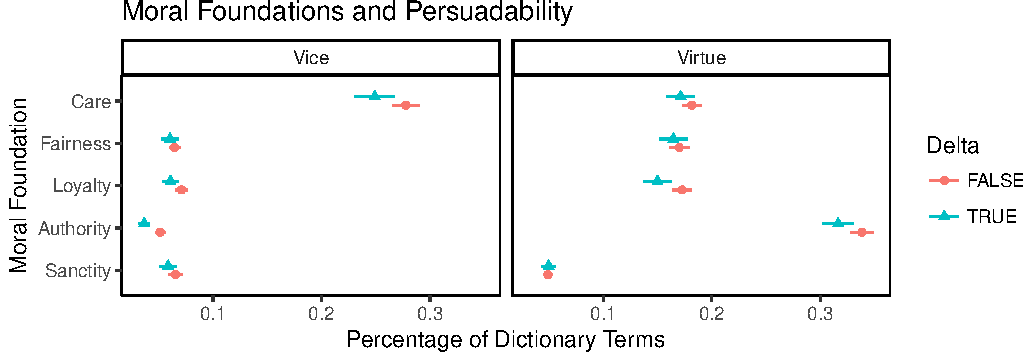
\includegraphics{prelim_files/figure-latex/examine op data-1.pdf}
\caption{Average percentage of dictionary terms relative to the total
number of words in each original post starting a discussion (including
95\% confidence intervals). Deltas indicate whether the author was
persuaded to change his or her view as a result of the discussion.}
\end{figure}

\section{Is Moral Consistency
Convincing?}\label{is-moral-consistency-convincing}

\begin{figure}
\centering
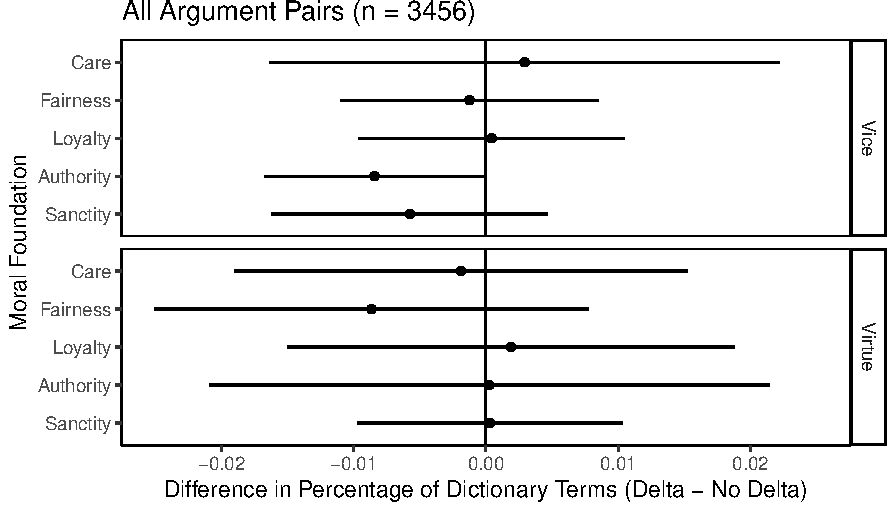
\includegraphics{prelim_files/figure-latex/check all discussion pairs-1.pdf}
\caption{All argument pairs: Average difference in percentage of
dictionary terms relative to the total number of words between matched
discussion contributions that persuaded the author of the original post
vs.~not (including 95\% confidence intervals). Negative values indicate
that arguments were less persuasive (and vice versa).}
\end{figure}

\begin{figure}
\centering
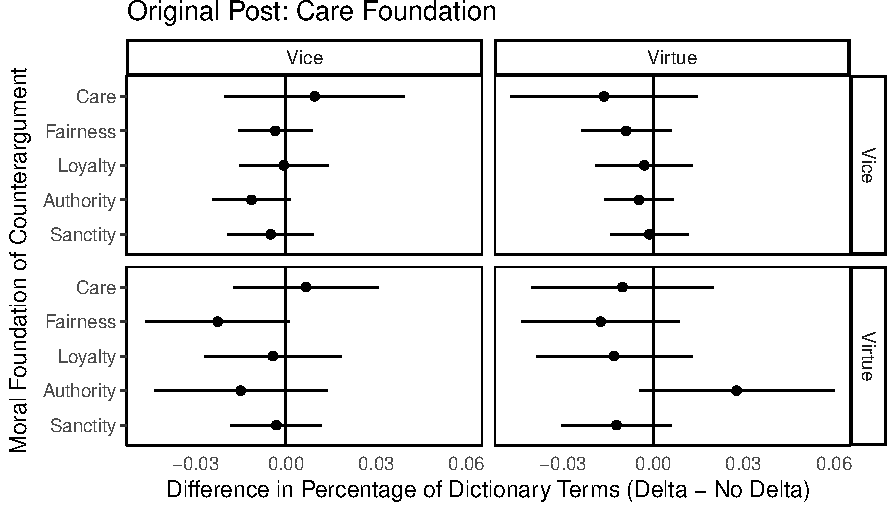
\includegraphics{prelim_files/figure-latex/harm virtue-1.pdf}
\caption{Care (virtue): Average difference in percentage of dictionary
terms relative to the total number of words between matched discussion
contributions that persuaded the author of the original post vs.~not
(including 95\% confidence intervals). Negative values indicate that
arguments were less persuasive (and vice versa).}
\end{figure}

\begin{figure}
\centering
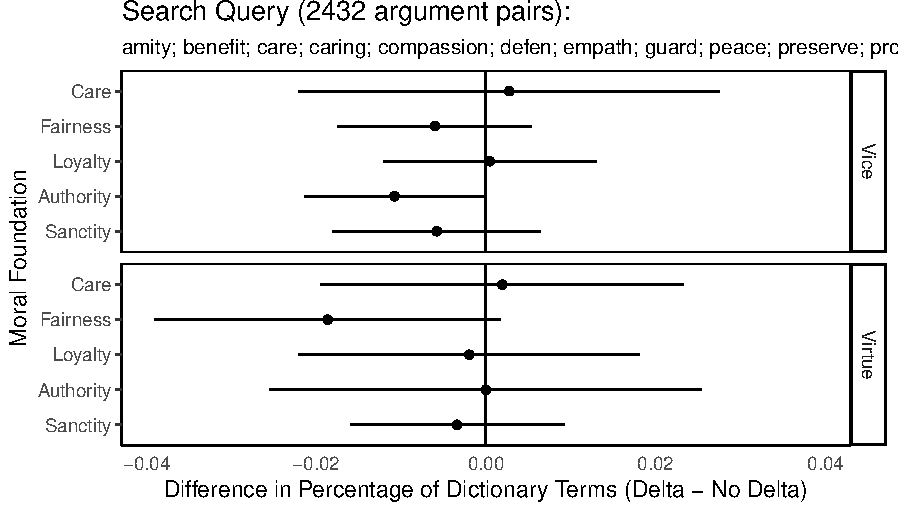
\includegraphics{prelim_files/figure-latex/harm vice-1.pdf}
\caption{Care (vice): Average difference in percentage of dictionary
terms relative to the total number of words between matched discussion
contributions that persuaded the author of the original post vs.~not
(including 95\% confidence intervals). Negative values indicate that
arguments were less persuasive (and vice versa).}
\end{figure}

\begin{figure}
\centering
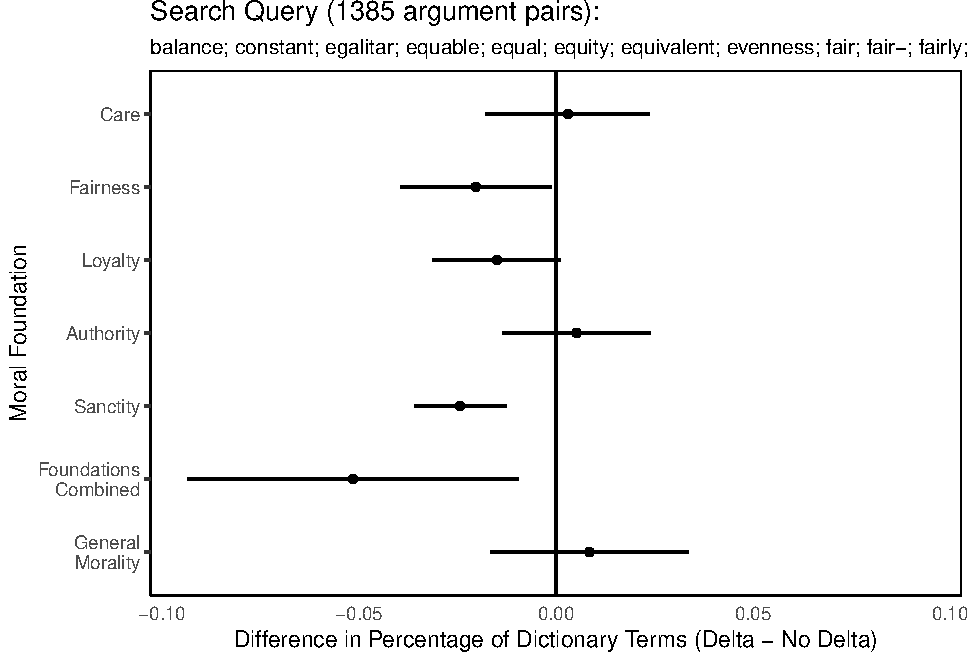
\includegraphics{prelim_files/figure-latex/fairness virtue-1.pdf}
\caption{Fairness (virtue): Average difference in percentage of
dictionary terms relative to the total number of words between matched
discussion contributions that persuaded the author of the original post
vs.~not (including 95\% confidence intervals). Negative values indicate
that arguments were less persuasive (and vice versa).}
\end{figure}

\begin{figure}
\centering
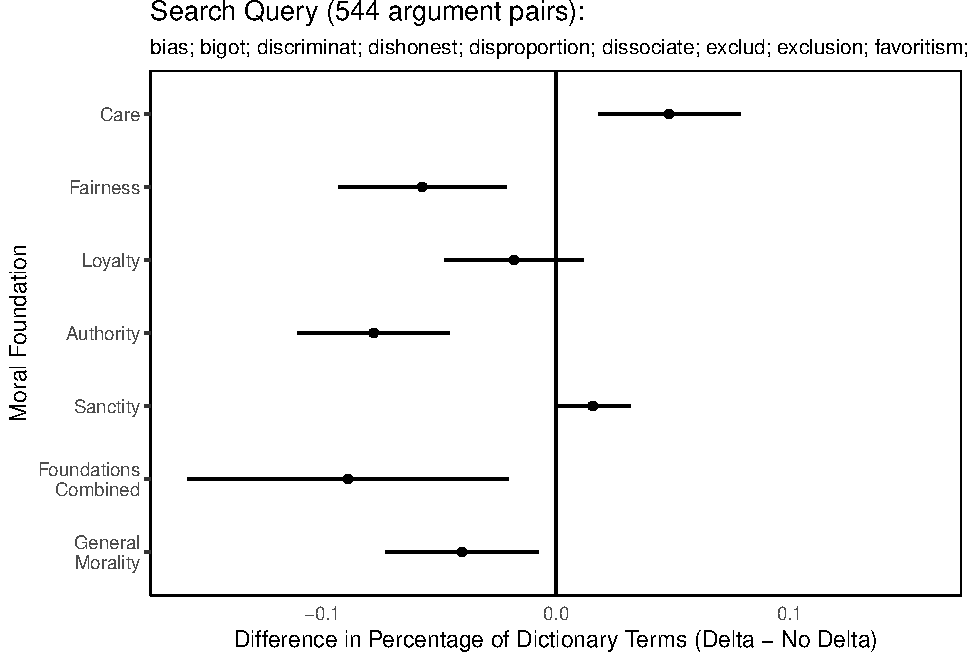
\includegraphics{prelim_files/figure-latex/fairness vice-1.pdf}
\caption{Fairness (vice): Average difference in percentage of dictionary
terms relative to the total number of words between matched discussion
contributions that persuaded the author of the original post vs.~not
(including 95\% confidence intervals). Negative values indicate that
arguments were less persuasive (and vice versa).}
\end{figure}

\begin{figure}
\centering
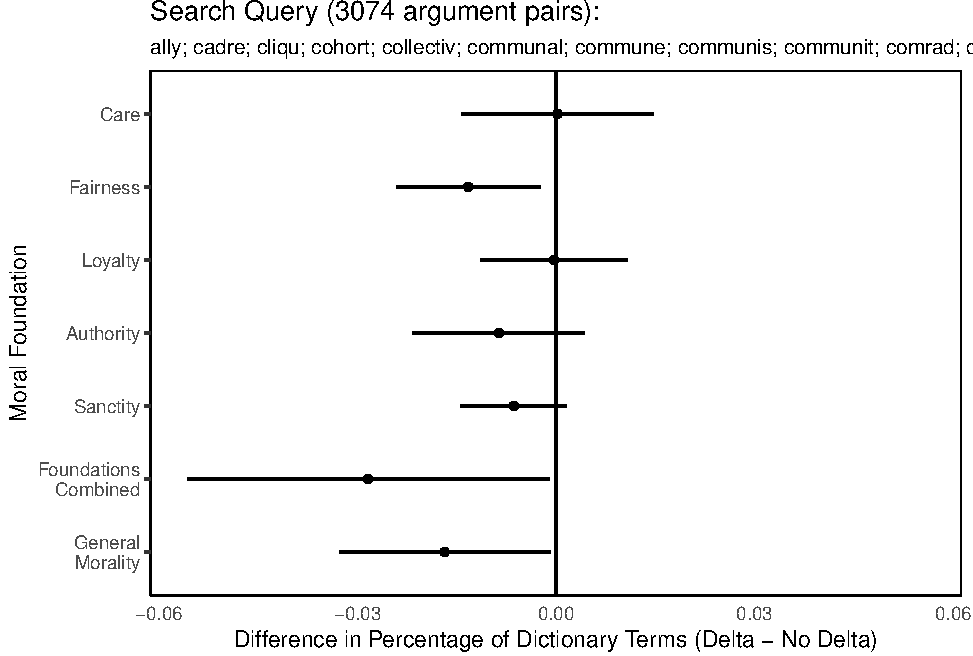
\includegraphics{prelim_files/figure-latex/ingroup virtue-1.pdf}
\caption{Loyalty (virtue): Average difference in percentage of
dictionary terms relative to the total number of words between matched
discussion contributions that persuaded the author of the original post
vs.~not (including 95\% confidence intervals). Negative values indicate
that arguments were less persuasive (and vice versa).}
\end{figure}

\begin{figure}
\centering
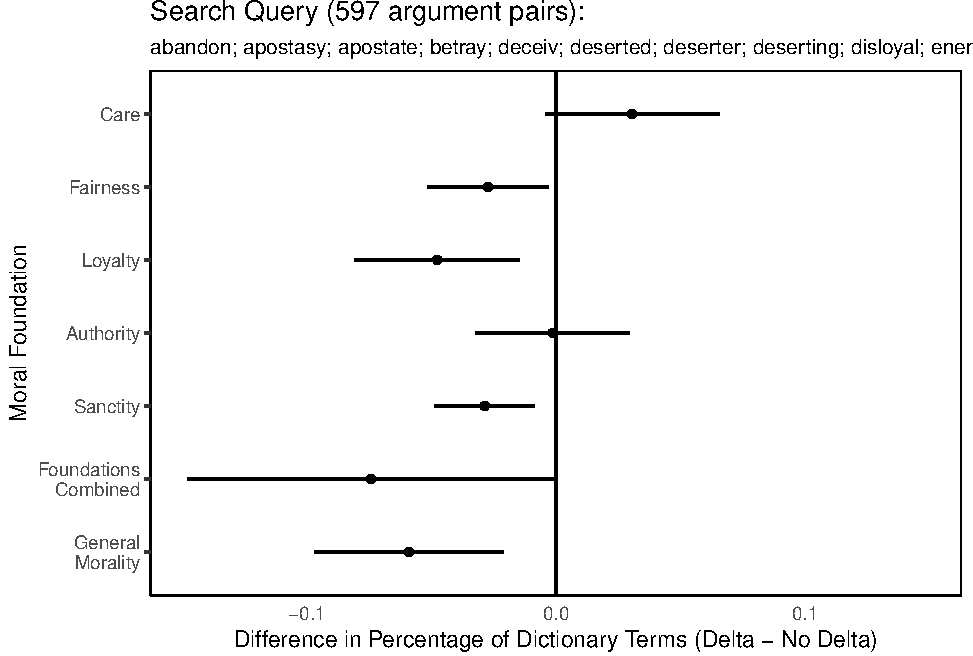
\includegraphics{prelim_files/figure-latex/ingroup vice-1.pdf}
\caption{Loyalty (vice): Average difference in percentage of dictionary
terms relative to the total number of words between matched discussion
contributions that persuaded the author of the original post vs.~not
(including 95\% confidence intervals). Negative values indicate that
arguments were less persuasive (and vice versa).}
\end{figure}

\begin{figure}
\centering
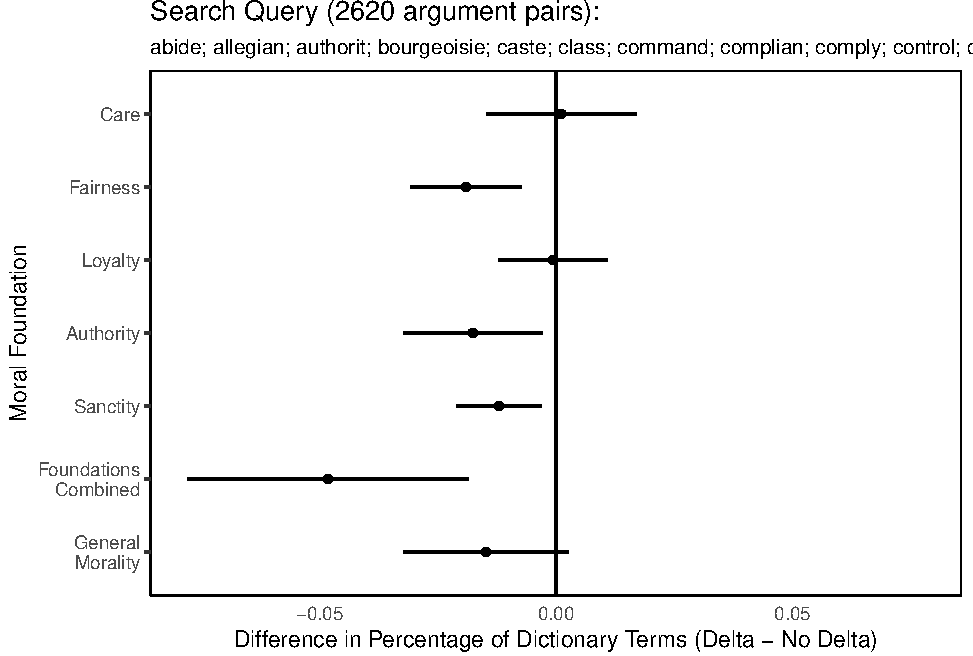
\includegraphics{prelim_files/figure-latex/authority virtue-1.pdf}
\caption{Authority (virtue): Average difference in percentage of
dictionary terms relative to the total number of words between matched
discussion contributions that persuaded the author of the original post
vs.~not (including 95\% confidence intervals). Negative values indicate
that arguments were less persuasive (and vice versa).}
\end{figure}

\begin{figure}
\centering
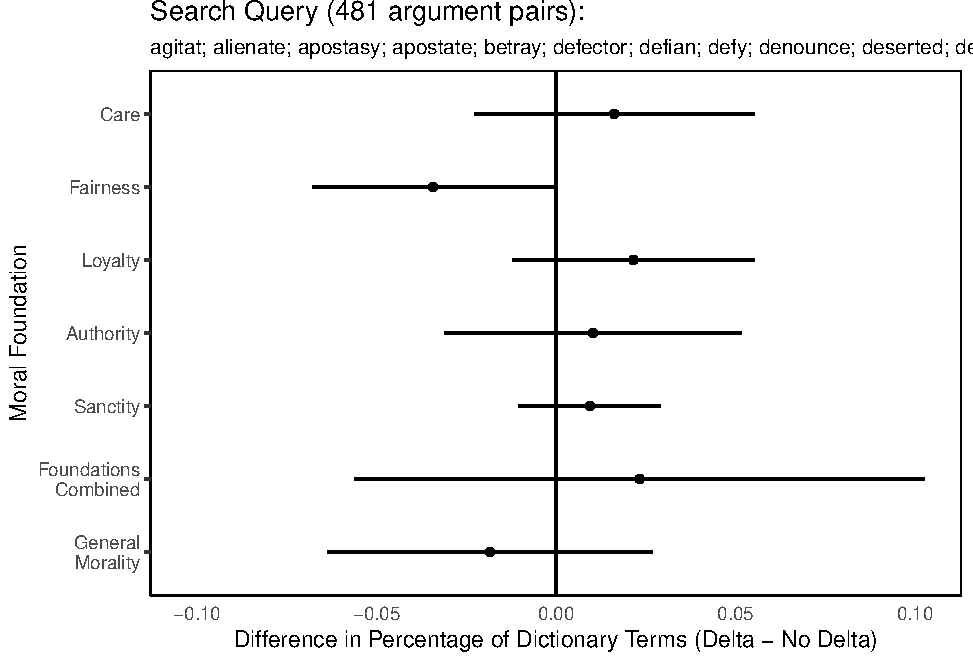
\includegraphics{prelim_files/figure-latex/authority vice-1.pdf}
\caption{Authority (vice): Average difference in percentage of
dictionary terms relative to the total number of words between matched
discussion contributions that persuaded the author of the original post
vs.~not (including 95\% confidence intervals). Negative values indicate
that arguments were less persuasive (and vice versa).}
\end{figure}

\begin{figure}
\centering
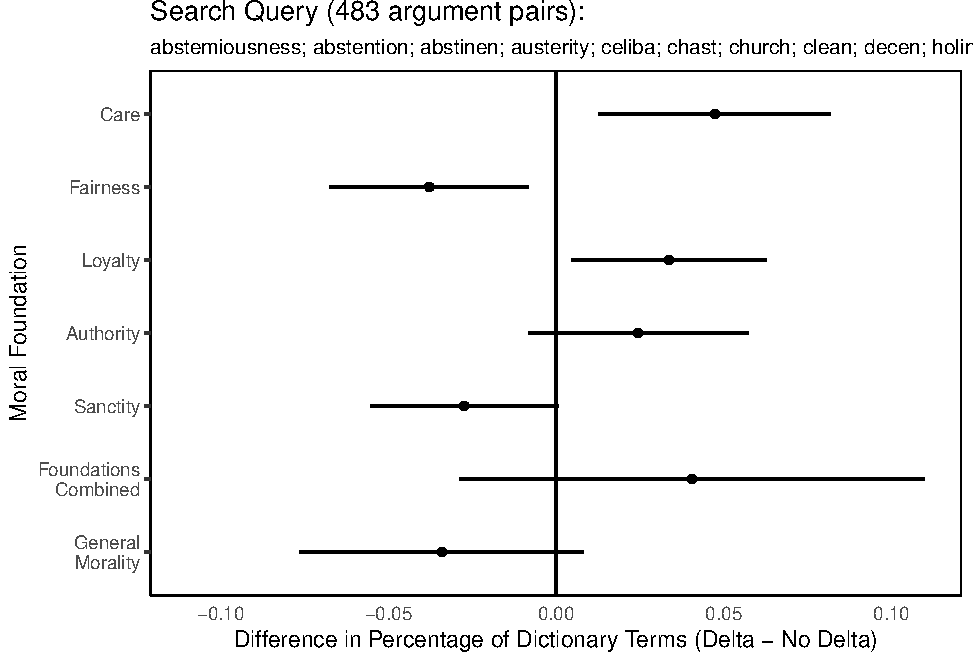
\includegraphics{prelim_files/figure-latex/purity virtue-1.pdf}
\caption{Sanctity (virtue): Average difference in percentage of
dictionary terms relative to the total number of words between matched
discussion contributions that persuaded the author of the original post
vs.~not (including 95\% confidence intervals). Negative values indicate
that arguments were less persuasive (and vice versa).}
\end{figure}

\begin{figure}
\centering
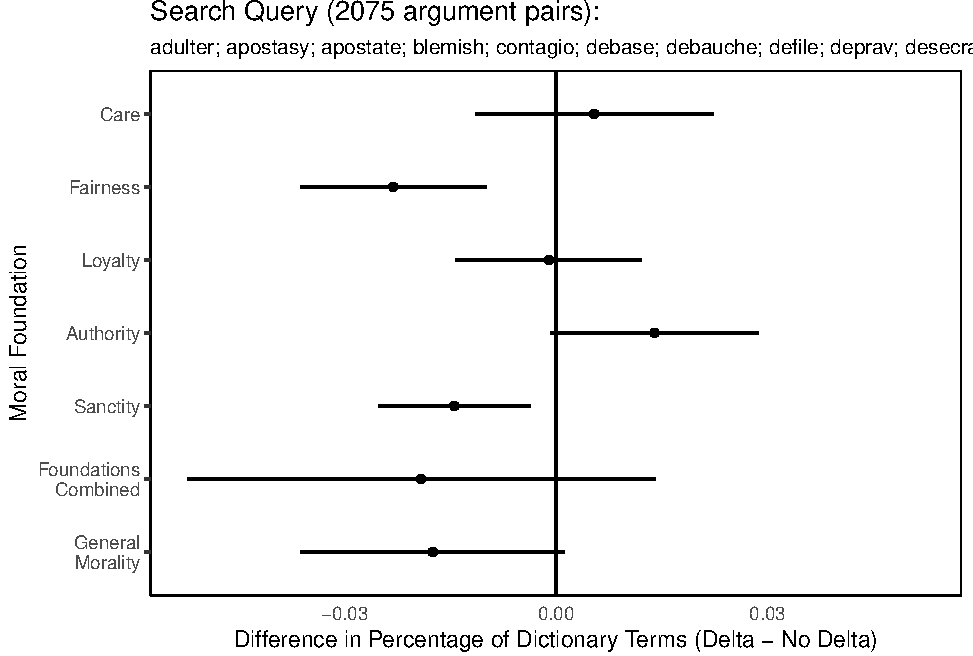
\includegraphics{prelim_files/figure-latex/purity vice-1.pdf}
\caption{Sanctity (vice): Average difference in percentage of dictionary
terms relative to the total number of words between matched discussion
contributions that persuaded the author of the original post vs.~not
(including 95\% confidence intervals). Negative values indicate that
arguments were less persuasive (and vice versa).}
\end{figure}

\clearpage

\section{Conclusion}\label{conclusion}

The preliminary results are consistent with the literature on moral
conviction and clearly contradict the implicit assumptions made in the
Moral Foundations literature. Overall, arguments that revolve around the
same moral foundations are less likely to be persuasive. In most cases,
moral appeals of any type appear counterproductive in facilitating
compromise and changing people's minds.

\section{TO DOs, future directions,
etc.}\label{to-dos-future-directions-etc.}

\begin{itemize}
\tightlist
\item
  examine specific topics (e.g., climate change etc.)
\item
  clean original posts (links etc)
\item
  adjust confidence intervals to correct for multiple comparisons
\item
  improve code documentation, add comments in internal functions
\item
  check MFT scores in argument pairs (as well as OP entry)
\end{itemize}




\newpage
\singlespacing 
\bibliography{/home/patrick/Dropbox/Uni/Lit/Literature}

\end{document}
